\section{Webanalysetools und Datenschutz}
Da das Einsetzen von Webanalyse Tools unumgänglich das Sammeln von Benutzerdaten bedeutet, ist die Handhabung dieser Daten von hoher Wichtigkeit. Analysetools verfolgen verschiedene Strategien, den Datenschutz zu gewährleisten. Dieses Kapitel veranschaulicht, wie Die Gesetzgebung auf verschiedenen Ebenen aussieht. Zudem wird erläutert, welche Kriterien ein Webanalysetool erfüllen sollte, um für den Einsatz im Verwaltungskontext in Erwägung gezogen zu werden.

\section{Typen von Webanalyse}

Webanalyse lässt sich aufgrund von verschiedenen Charakteristiken Gruppieren \parencite[S. 172-174]{nakatani2011toolselectionmethod}.

\begin{description}
  \item[Methode der Datensammlung] Bezieht sich auf die technische Art wie die Daten gesammelt werden. Dazu gehören: Web Beacon, Packet Sniffing, Transaktionsloganalyse und Page Tagging.  
  \item[Art des Zugriffs auf den Service] Erklärt die Bereitstellung des Aufzeichnungs- und Analyseservices. Dazu zählen: Software as a Service (SaaS), Application Service Provider und In-House.
  \item[Typ des zu verfolgenden Gerätes/Systems] Beinhaltet die Arten der Zielsystemen welche analysiert werden können. Beispiele für solche Systeme sind: Mobilgeräte, Browser oder Nativ-Applikationen.
  \item[Datenverfügbarkeit und Geschwindigkeit] Bezieht sich auf die Unterschiede in der Geschwindigkeit beim Bereitstellen der aufgezeichneten Daten. Einige Tools ermöglichen Analysen in Echtzeit, während andere Minuten bis zu Stunden brauchen um die Daten aufzubereiten.
\end{description}

Anhand der Gruppierung auf Basis der Methode der Datensammlung lässt sich ein guter Überblick an Tools auf dem Markt schaffen. Die Datensammlung lässt sich im wesentlichen auf vier verschiedene Arten durchführen, wobei Transaktionsloganalyse und Page Tagging als die am häufigsten eingesetzten Tools gelten \parencite{nakatani2011toolselectionmethod}.

\subsection{Web Beacon} 
Bei Web Beacons handelt es sich um kleine Bilddateien, welche sich auf einer Webseite eingefügt werden können und per Request angefordert werden \parencite[S. 173]{nakatani2011toolselectionmethod}. Web Beacons werden in der Praxis nur noch selten eingesetzt. Sie Werden hauptsächlich dafür verwendet, Kundenverhalten über mehrere Webseiten hinweg zu verfolgen. Eine der Häufigsten Applikationen ist das Bewerten der Leistung von Bannerwerbung. Für einfache Webanalyse wird diese Methode eher selten verwendet \parencite[S. 3]{waisberg2009webShort}.

\subsection{Packet Sniffing}
Durch das Abfangen und analysieren der Webpakete auf dem Webserver, können mit Packet Sniffing Daten gesammelt werden. Packet Sniffing findet in der Praxis hauptsächlich Anwendung bei multivariatem Testen \parencite[S. 4]{waisberg2009webShort}.

% TODO Packet Sniffing


\subsection{Transaktionsloganalyse} 
Bei dieser Methode werden die Log Dateien auf dem Webserver analysiert. Transaktionsloganalyse ist eine in der Praxis nach wie vor verwendete Methode, um Daten über Webseitenaufrufe zu sammeln.\parencite[S. 173]{nakatani2011toolselectionmethod}. Die Tiefe der Daten die gesammelt werden können hält sich jedoch im Vergleich zu anderen Methoden in Grenzen. Es lassen sich durch Transaktionsloganalyse folgende Informationen Sammeln \parencite[S. 2]{waisberg2009webShort}:

\begin{description}
  \item[IP] Die IP-Adresse des Computers der die Webseite angefordert hat
  \item[Datum und Zeit] Zeitpunkt des Anfordern der Daten
  \item[Verarbeitungszeit] Wie lange die Transaktion gedauert hat
  \item[Grösse] Anzahl Bytes die übertragen wurden
\end{description}

Ausserdem bietet Transaktionsloganalyse gegenüber den anderen Methoden die folgenden Vorteile\parencite[S. 2]{waisberg2009webShort}:

\begin{description}
  \item[Dateneigentum] Der Besitzer der Webseite ist ebenfalls der Besitzer der Logs und somit der gesammelten Daten. 
  \item[Rückwärts Verfügbarkeit] Die Daten in den Logs können, solange sie gespeichert bleiben, erneut analysiert und verarbeitet werden. 
  \item[Speichert Verhalten von Crawler] Da auch Hits von Crawler Transaktionen sind, werden diese in den Logs gespeichert. Sie sind zwar nicht notwendig für die Analyse der menschlichen Aktivitäten, doch sind sie wichtig für die Suchmaschienenoptimierung\parencite[S. 174]{nakatani2011toolselectionmethod}. 
\end{description}


\subsection{Page Tagging} 
Page Tagging ist die Sammlung der Daten von Webseitenbesucher durch ein JavaScript-File auf jeder Webseite. Dieses JavaScript-File zeichnet das Verhalten des Seitenbesuchers auf, und sendet die Informationen an einen zentralen Datensammlungsserver \parencite[S. 173]{nakatani2011toolselectionmethod}. PageTagging ermöglichte es, im Gegensatz zu Transaktionsloganalyse, detaillierter Daten aufzuzeichnen. Da das JavaScript-Programm lokal auf dem Computer des Webseitenbesuchers ausgeführt wird, ist die Art der Daten die gesammelt werden können beinahe unbegrenzt. Durch das Modifizieren des JavaScript-Codes, kann beliebig angepasst werden, welche Daten das gesammelt werden sollen. Ausserdem bietet Transaktionsloganalyse gegenüber den anderen Methoden die folgenden Vorteile\parencite[S. 174]{nakatani2011toolselectionmethod}:

\begin{description}
  \item[Präzision] Page Tagging zählt alle Hits die durch Webbrowser ausgeführt werden. Durch das ausführen des JavaScript-Programm werden auch wenn die Seite im Cache ist die Hits gezählt.
  \item[Client-Side Aktivitäten] Durch die Gegebenheit, dass Page Tagging lokal ausgeführt wird, können nebst Seitenaufrufen weitere Daten aufgezeichnet werden.
  \item[Wiederkehrende Besucher] Durch den Einsatz von Cookies, kann mittels Page Tagging einfach herausgefunden werden, ob es sich um neue oder wiederkehrende Besucher handelt.
  \item[Outsourcing] Page Tagging wird üblicherweise in Form eines Services angeboten. Organisationen, welche nicht über die Infrastruktur verfügen In-House Analysen durchzuführen sind auf solche Services angewiesen.
\end{description}

Die Umfrage (Anhang \ref{appendix:umfrage}) hat ergeben, dass 100\% der Befragten, die Webanalyse betreiben, ein Webanalysetool einsetzen, welches die Methode des Page Tagging verwendet. Aus diesem Grund, wird die Analyse des Marktangebotes auf die Webanalysetools dieser Methode eingeschränkt.

\section{Marktangebot - Webanalysetools}
Auch durch Einschränken des Marktes auf Webanalysetools der Methode Page Tagging, gibt es eine riesige Menge an Tools die auf dem Markt verfügbar sind. Gemäss \parencite{datanyzeSwitzerlandWebanalytics}, sind in der Schweiz ~129 verschiedene Webanalysetools im Einsatz. Dabei macht Google Analytics mit Abstand den grössten Teil aus. Über 70\% des Marktes verwendet Google Analytics (GA). Obwohl es in der Umfrage (siehe Anhang \ref{appendix:umfrage}) nicht erschien, ist mit nur knapp 3.5\% ist Facebook Analytics (FA) der zweit grösste Anbieter am Markt. Matomo (M) Ist der am Schweizer Markt dritt grösste Anbieter. Matomos Marktanteil beträgt 2.8\%. Hotjars (J) Marktanteil ist 1.2\%, während sich Monster Insights (MI) Marktanteil auf 0.9\% beläuft. 

\begin{figure}[h]
  \centering
  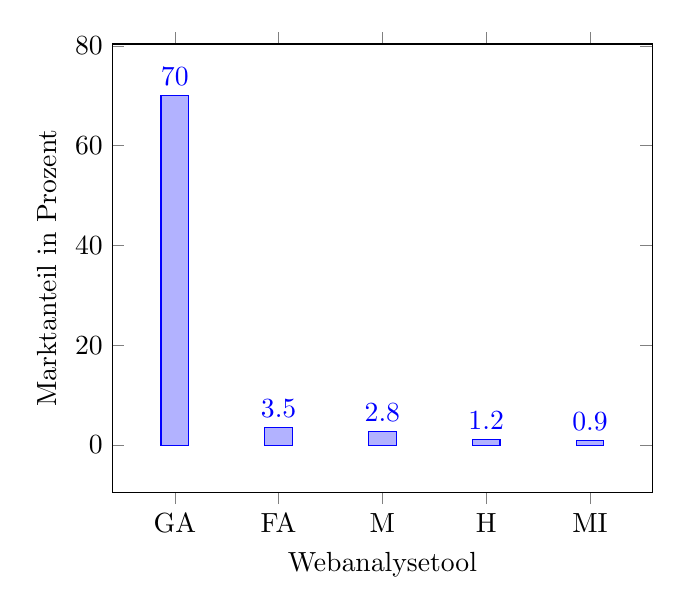
\begin{tikzpicture}  
    \begin{axis}  
    [  
        ybar,  
        enlargelimits=0.15,  
        ylabel={Marktanteil in Prozent}, % the ylabel must precede a # symbol.  
        xlabel={Webanalysetool},  
        symbolic x coords={GA, FA, M, H, MI}, % these are the specification of coordinates on the x-axis.  
        xtick=data,  
         nodes near coords, % this command is used to mention the y-axis points on the top of the particular bar.  
        nodes near coords align={vertical},  
        ]  
    \addplot coordinates {(GA,70) (FA,3.5) (M,2.8) (H,1.2) (MI,0.9)};  
    \end{axis}  
    \end{tikzpicture}  
  \caption{Marktanteile der Webanalysetools in der Schweiz \parencite{datanyzeSwitzerlandWebanalytics}}
  \label{fig:marktanteil}
\end{figure}

\subsection{Google Analytics}
Google Analytics ist sowohl in der Schweiz als auch Global das am meisten eingesetzten Webanalyse Tool \parencite{datanyzeSwitzerlandWebanalytics}.  

\subsection{Facebook Analytics}

\subsection{Matomo}

\subsection{i-CMS}
Bei i-CMS handelt es sich an sich nicht um ein Webanalysetool, sondern um ein Produkt-Paket der Firma Innovative Web AG. Es ist ein Webauftritt-Paket, Welches sowohl die Grundfunktionalitäten eines CMS, als auch Web- und Businesstatistik zur Verfügung stellt\parencite{iwebwebsiteCMS}. Wie die Grafik \ref{fig: icms} zeigt, kann spezifische Module das Tool auf Wunsch des Kunden erweitert werden.


\begin{figure}[h]
  \centering
  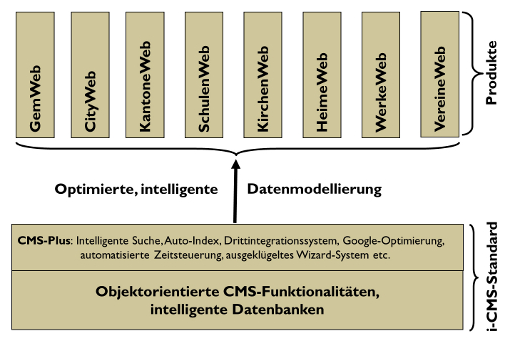
\includegraphics[width=9cm]{icms.png}
  \caption{i-CMS Modularität \parencite{iweb2019revue}}
  \label{fig: icms}
\end{figure}

Diese Modularität ermöglicht es ein breites Spektrum an Kunden zu bedienen, wobei das Angebot immer auf den Kunden zugeschnitten bleibt. Dabei liegt der Fokus der Zielgruppe auf Verwaltungen und Vereinen. Es lassen sich Module für Städte, Gemeinden sowie Kantone einbinden. Beispielsweise beim Modul KantonWeb stehen zusätzlich zu den üblichen CMS-Funktionen ebenfalls Kantonsspezifische Module wie zum Beispiel die kantonale Rechtspflege eingebunden werden \parencite{iwebwebsiteKanotonWeb}. Dies macht die i-CMS-Plattform zu einer attraktiven Lösung für den Webauftritt jeglicher Verwaltungen. 

I-web gibt auf ihrer Webseite \parencite{iwebwebsiteKanotonWeb} an, dass i-CMS und sämtliche Erweiterungsmodule Datenschutz konform sind. Dies wird dadurch erreicht, dass alle Webseiten die das i-CMS verwenden eine Einwilligung durch den Benutzer erfordern, die Datenschutzbestimmungen zu akzeptieren. Wie auf der Abbildung \ref{fig: urweb} zu sehen ist, geschieht die Einwilligung durch einen Knopfdruck auf "Ja" zu der Frage: "Dürfen wir Ihre anonymisierten Daten verwenden?". Es werden weitere Massnahmen unternommen, die Daten der Benutzer so gut wie möglich zu schützen. Die Verarbeitung der Daten findet laut Innovative Web AG \parencite{iwebwebsiteCMS} ausschliesslich in der Schweiz statt (siehe auch Abbildung \ref{fig: urweb}) und werden anonymisiert gehalten. Es können aus den gesammelten Daten der Statistik also keine Rückschlüsse auf einzelne Personen gezogen werden. 

\begin{figure}[h]
  \centering
  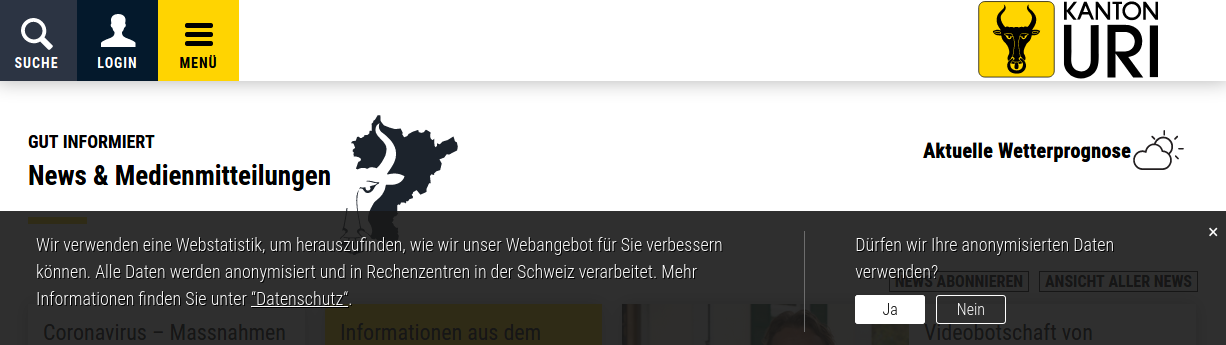
\includegraphics[width=15cm]{ur-website.png}
  \caption{Webseite des Kanton Uri \parencite{webseiteKantonUri}}
  \label{fig: urweb}
\end{figure}

I-CMS wird von einigen Gemeinde-, Stadt- und Kantonsverwaltungen eingesetzt. In der unten stehenden Grafik \ref{fig: iwebmap2019} wird veranschaulicht, in welchen Gebieten der Schweiz i-CMS überall zum Einsatz kommt. Rot markiert sind die Gemeinden, in welchen ein Webauftritt mittels i-CMS eingeführt wurde. Gemäss \parencite[S. 14]{iweb2018revue}, waren es im August 2018 über 800 Kunden, davon ungefähr 550 Gemeinde und Stadtverwaltungen \parencite{iwebwebsiteGemeindeWeb}.

\begin{figure}[h]
  \centering
  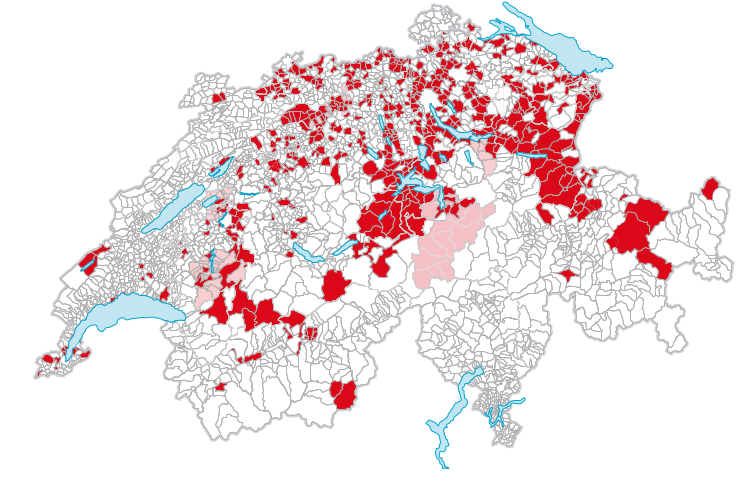
\includegraphics[width=9cm]{iweb-map-2019.png}
  \caption{i-web Marktpräsenz \parencite[S. 14]{iweb2019revue}}
  \label{fig: iwebmap2019}
\end{figure}

Als es in den Beiden Jahren 2017 und 2018 danach aussah, als würde sich i-CMS am Markt verdrängen lassen, kam i-CMS mit einem Starken Jahr zurück (siehe Grafik \ref{fig:icmszuwachs}). Dies lässt darauf schliessen, dass die Popularität von i-CMS bei den Verwaltungen nicht nachgelassen hat.

% TODO aussagen zum Webanalysetool von I-CMS

\begin{figure}[h]
  \centering
  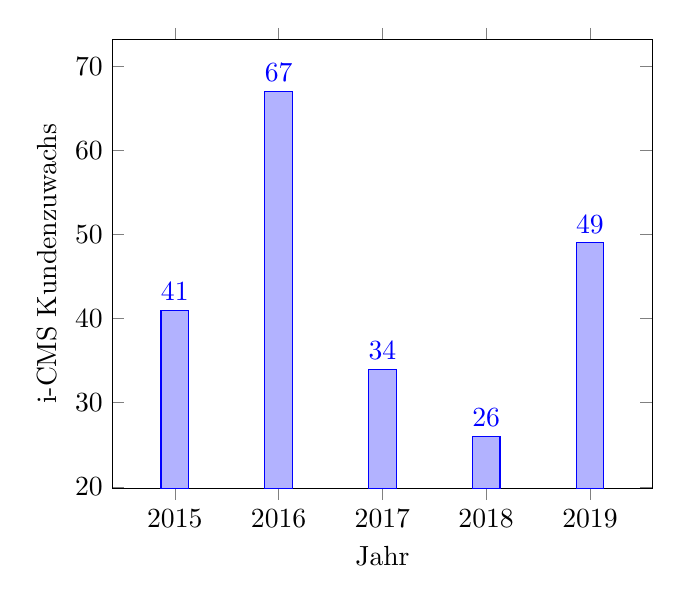
\begin{tikzpicture}  
    \begin{axis}  
    [  
        ybar,  
        enlargelimits=0.15,  
        ylabel={i-CMS Kundenzuwachs}, % the ylabel must precede a # symbol.  
        xlabel={Jahr},  
        symbolic x coords={2015, 2016, 2017, 2018, 2019}, % these are the specification of coordinates on the x-axis.  
        xtick=data,  
         nodes near coords, % this command is used to mention the y-axis points on the top of the particular bar.  
        nodes near coords align={vertical},  
        ]  
    \addplot coordinates {(2015,41) (2016,67) (2017,34) (2018,26) (2019,49)};  
    \end{axis}  
    \end{tikzpicture}  
  \caption{Kundenzuwachs i-CMS \parencite[S. 14]{iweb2015revue}, \parencite[S. 14]{iweb2016revue}, \parencite[S. 14]{iweb2017revue}, \parencite[S. 14]{iweb2018revue}, \parencite[S. 14]{iweb2019revue}}
  \label{fig:icmszuwachs}
\end{figure}

\subsection{Erwähnenswerte Tools}

\section{Vorgehen der Tool-Auswahl}


